\chapter{Language popularity} \label{appendix:langpop}

\section{PopularitY of Programming Languages (PYPL)}\ftnt{http://pypl.github.io/PYPL.html}
The PYPL index uses Google trends\ftnt{https://www.google.com/trends/} as a leading indicator of the popularity of a programming language.
It search for the trend for each programming language by counting the number of searches of this language and the word "tutorial".



PYPL for May 2015\\
\begin{tabular}{c c l r r}
Rank & Change              & Language        & Share  & Trend   \\ \hline
1    &                     & Java            & 24.1\% & -0.9\%  \\ \hline
2    &                     & PHP             & 11.4\% & -1.6\%  \\ \hline
3    &                     & Python          & 10.9\% & +1.3\%  \\ \hline
4    &                     & C\#             & 8.9\%  & -0.7\%  \\ \hline
5    &                     & C++             & 8.0\%  & -0.2\%  \\ \hline
6    &                     & C               & 7.6\%  & +0.2\%  \\ \hline
7    &                     & Javascript      & 7.1\%  & -0.6\%  \\ \hline
8    &                     & Objective-C     & 5.7\%  & -0.2\%  \\ \hline
9    &                     & Matlab          & 3.1\%  & +0.1\%  \\ \hline
10   & $2\times\uparrow$   & R               & 2.8\%  & +0.7\%  \\ \hline
11   & $5\times\uparrow$   & Swift           & 2.6\%  & +2.9\%  \\ \hline
12   & $1\times\downarrow$ & Ruby            & 2.5\%  & +0.0\%  \\ \hline
13   & $3\times\downarrow$ & Visual Basic    & 2.2\%  & -0.6\%  \\ \hline
14   & $1\times\downarrow$ & VBA             & 1.5\%  & -0.1\%  \\ \hline
15   & $1\times\downarrow$ & Perl            & 1.2\%  & -0.3\%  \\ \hline
16   & $1\times\downarrow$ & lua             & 0.5\%  & -0.1\%  \\ \hline
\end{tabular}



\section{TIOBE}\ftnt{http://www.tiobe.com/index.php/content/paperinfo/tpci/index.html}

The TIOBE index uses many search engines as an indicator of the current popularity of programming languages.
It count the number of pages each search engine find when queried with the language name and the word "programming".
This indicator indicates the number of resources available, and the discussions about a given programming language.

Javascript was the most rising language of 2014 in the TIOBE index.

TIOBE for April 2015\\
\begin{tabular}{c c c l r r}
Apr 2015 & Apr 2014 & Change           & Programming Language & Ratings  & Change  \\ \hline
1        & 2        & $\uparrow$       & Java                 & 16.041\% & -1.31\%  \\ \hline
2        & 1        & $\downarrow$     & C                    & 15.745\% & -1.89\%  \\ \hline
3        & 4        & $\uparrow$       & C++                  & 6.962\%  & +0.83\%  \\ \hline
4        & 3        & $\downarrow$     & Objective-C          & 5.890\%  & -6.99\%  \\ \hline
5        & 5        &                  & C\#                  & 4.947\%  & +0.13\%  \\ \hline
6        & 9        & $\uparrow$       & JavaScript           & 3.297\%  & +1.55\%  \\ \hline
7        & 7        &                  & PHP                  & 3.009\%  & +0.24\%  \\ \hline
8        & 8        &                  & Python               & 2.690\%  & +0.70\%  \\ \hline
9        & -        & $2\times\uparrow$ & Visual Basic        & 2.199\%  & +2.20\%  \\ \hline
\end{tabular}



\section{Programming Language Popularity Chart}\ftnt{http://langpop.corger.nl}

The programming language popularity chart indicates the activity of a given language in the online communities.
It uses two indicators to rank languages : the number of line changed in github of, and the number of questions tagged with a certain language.

% \includesvg{../../data/js-trends/langpop-5may15}

Javascript is ranked number one in this index.
The Javascript community is particularly active online, and in the open source.



% Stack overflow tags
% http://makingdataeasy.com/stackoverflow-trends?tc=relative-button


% Github repo
% http://adambard.com/blog/top-github-languages-2014/
% https://bigquery.cloud.google.com/table/githubarchive:github.timeline?pli=1

indeed.com
% http://www.indeed.com/jobtrends/javascript+developer%2C+java+developer%2C+sql+developer%2C+c%2B%2B+developer%2C+ruby+developer%2C+ios+developer%2C+c%23+developer%2C+python+developer%2C+c+developer%2C+php+developer.html


\section{Black Duck Knowledge}\ftnt{https://www.blackducksoftware.com/resources/data/this-years-language-use}

The black-duck, which analyze the usage of language on many forges, and collaborative hosts, rank Javascript number 2, after C, and with about the same usage as C++.

github.com 
sourceforge.net 
cpan.org 
rubyforge7.org 
planetsourcecode.com 
ddj.com

\begin{tabular}{l r}
Language     & \%     \\ \hline\hline
C            & 34.80  \\ \hline
Javascript   & 15.45  \\ \hline
C++          & 15.13  \\ \hline
Java         & 14.02  \\ \hline
PHP          & 2.87   \\ \hline
Autoconf     & 2.65   \\ \hline
Python       & 2.15   \\ \hline
Ruby         & 1.77   \\ \hline
XML Schema   & 1.73   \\ \hline
Shell        & 1.18   \\ \hline
Assembler    & 1.16   \\ \hline
SQL          & 1.07   \\ \hline
Make         & 0.94   \\ \hline
Perl         & 0.92   \\ \hline
C\#          & 0.90   \\ \hline
\end{tabular}

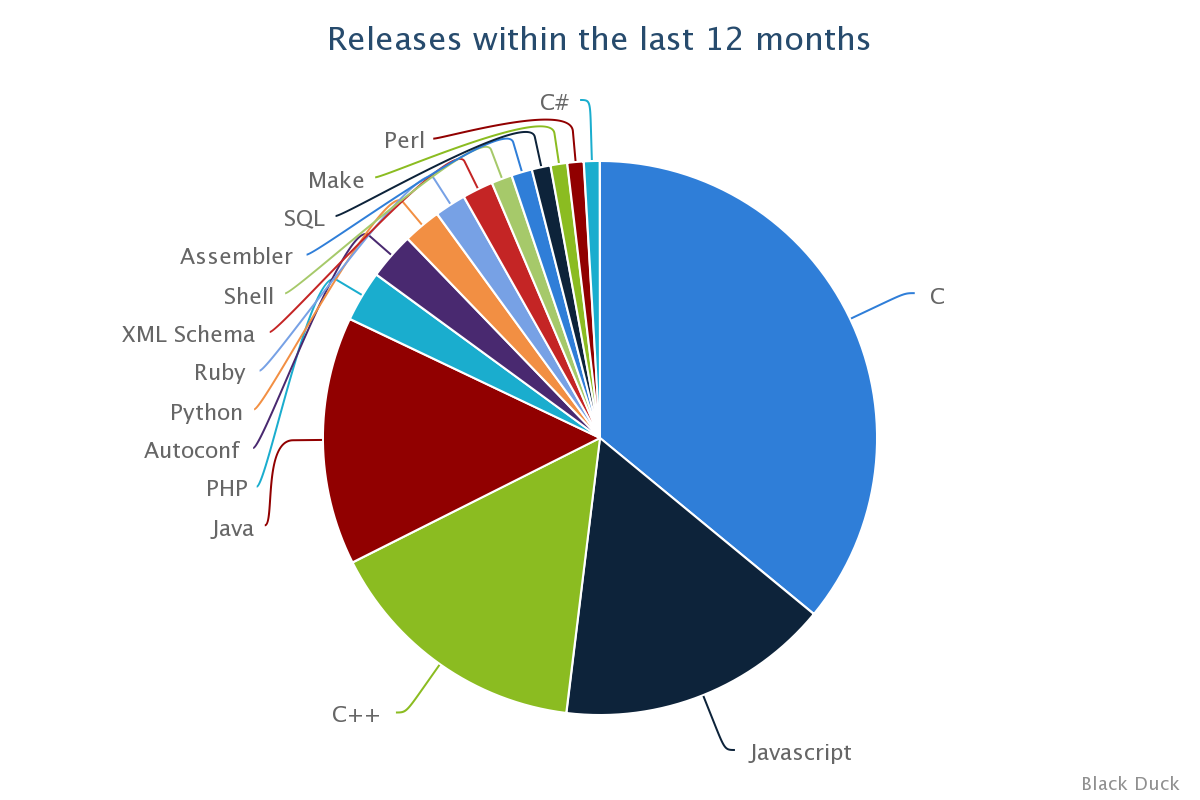
\includegraphics[width=\linewidth]{../../data/js-trends/black-duck-15}


\section{Github}

http://githut.info/



\section{HackerNews Poll}

https://news.ycombinator.com/item?id=3746692

\begin{tabular}{l r}
Language     & Count \\ \hline\hline
Python       & 3335 \\ \hline
Ruby         & 1852 \\ \hline
JavaScript   & 1530 \\ \hline
C            & 1064 \\ \hline
C\#          & 907 \\ \hline
PHP          & 719 \\ \hline
Java         & 603 \\ \hline
C++          & 587 \\ \hline
Haskell      & 575 \\ \hline
Clojure      & 480 \\ \hline
CoffeeScript & 381 \\ \hline
Lisp         & 348 \\ \hline
Objective C  & 341 \\ \hline
Perl         & 341 \\ \hline
Scala        & 255 \\ \hline
Scheme       & 202 \\ \hline
Other        & 195 \\ \hline
Erlang       & 171 \\ \hline
Lua          & 150 \\ \hline
Smalltalk    & 130 \\ \hline
Assembly     & 116 \\ \hline
SQL          & 112 \\ \hline
Actionscript & 109 \\ \hline
OCaml        & 88 \\ \hline
Groovy       & 83 \\ \hline
D            & 79 \\ \hline
Shell        & 76 \\ \hline
ColdFusion   & 51 \\ \hline
Visual Basic & 47 \\ \hline
Delphi       & 45 \\ \hline
Forth        & 41 \\ \hline
Tcl          & 34 \\ \hline
Ada          & 29 \\ \hline
Pascal       & 28 \\ \hline
Fortran      & 26 \\ \hline
Rexx         & 13 \\ \hline
Cobol        & 12 \\ \hline
\end{tabular}